\title{jeffery_lim}
\documentclass[11pt, a4paper]{article}
\usepackage[utf8]{inputenc}

\usepackage{listings}
\usepackage[framed,numbered,autolinebreaks,useliterate]{mcode}

\usepackage[margin=1in]{geometry}
\usepackage{graphicx}
\usepackage{amsmath}
\usepackage{float}
\graphicspath{ {../} }
\setlength\parindent{0pt}

\begin{document}

\begin{center}
  \Huge ECEN4532, DSP Laboratory \\
  \huge Homework \\
  
  \vspace{7in}
    \huge Jeffery Lim \\
    \huge Jeffery.Lim@colorado.edu\\~\\~\\
\end{center}
\pagebreak

The first few lines are loading the audio file and then runing the discrete cosine transform.

\lstinputlisting[language=Matlab, firstline=1, lastline = 5]{../workspace.m}

The next steps to sort the result were not followed. I did not find them necessary to follow. Instead, a threshold was determined and tested to find at what threshold the resulting reconstruction would give a .1\% rate. 


\lstinputlisting[language=Matlab, firstline=6, lastline = 15]{../workspace.m}

The number of coefficients removed due to the thresheold is 321. The remaining coefficients are 4578, or 93.45\%.

The resulting plots are as following. The image is when the amount of energy is 99.9\%. 

\lstinputlisting[language=Matlab, firstline=16, lastline = 30]{../workspace.m} 


\begin{figure}[H]
\hspace*{-2cm}    
    \centering
    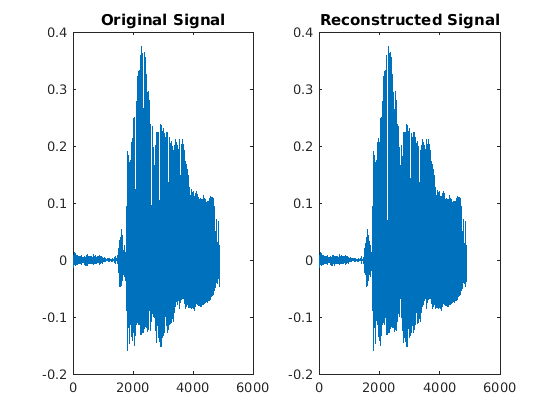
\includegraphics[width=\textwidth]{ReconstructedImage99.png}
    \caption{Reconstructed Song with .0004 Threshold}
\end{figure}

As evident in the image, there is a visibly exact match between the original and the reconstructed image. The other thresholds that were tested before have a visible difference and a signficiant difference. 


\begin{figure}[H]
\hspace*{-2cm}    
    \centering
    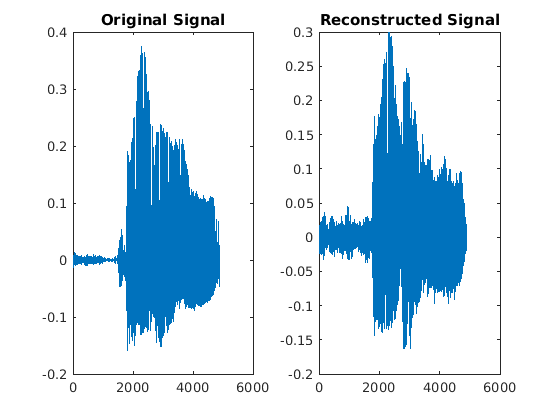
\includegraphics[width=\textwidth]{ReconstructedImage64.png}
    \caption{Reconstructed Song with .1 Threshold}
\end{figure}


\begin{figure}[H]
\hspace*{-2cm}    
    \centering
    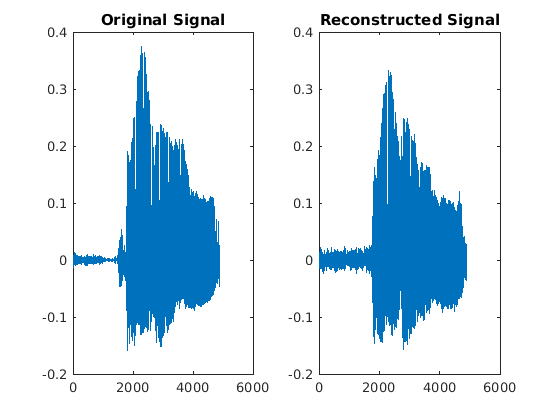
\includegraphics[width=\textwidth]{ReconstructedImage76.png}
    \caption{Reconstructed Song with .05 Threshold}
\end{figure}


\begin{figure}[H]
\hspace*{-2cm}    
    \centering
    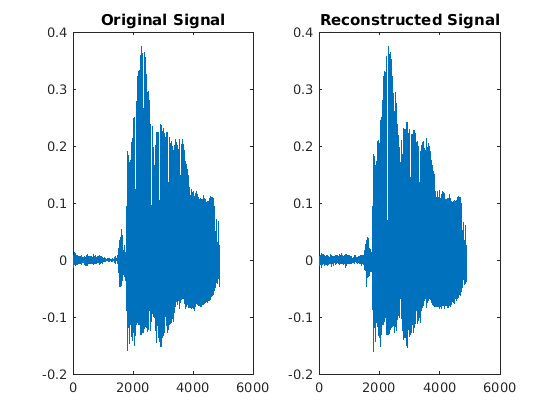
\includegraphics[width=\textwidth]{ReconstructedImage94.png}
    \caption{Reconstructed Song with .001 Threshold}
\end{figure}

\end{document}

